\documentclass[10pt]{article}
\usepackage[margin=0.72in]{geometry}
\usepackage{graphicx}
\usepackage{booktabs}
\usepackage{array}
\usepackage{hyperref}
\usepackage{xcolor}
\hypersetup{colorlinks=true,linkcolor=blue,urlcolor=blue}
\setlength{\parindent}{0pt}
\setlength{\parskip}{4pt}
\newcommand{\pass}{\textcolor{green!45!black}{PASS}}
\title{TX4 Exact P4 / GFL11 Julia Reproduction}
\author{IAS 2026 independent validation bundle}
\date{2026-09-20}

\begin{document}
\maketitle

\section*{Verdict}

The exact frozen TX4 P4 flagship closes as Case A for the requested custom same-model Python-vs-Julia reproduction. The independent Julia implementation reproduces the frozen Python V4 census with the exact 11-state GFL, exact P4 SG policy, matched AC equilibrium, 16-case verdict agreement, and critical voltage-mode MAC of $0.9999999999999988$ for H4.

This is an IAS poster-credibility upgrade for the stated same-model spectral claim. It is not an EMT, PowerDynamics SimpleGFLDC, or TPWRS-equivalence result.

\section*{Frozen setup}
\begin{itemize}
  \item H4: $\{30,33,35,37\}$.
  \item P4: $(g,k,t,h)=(0.03625,1.425,1.5,1.0)$.
  \item GFL11 order: $[\theta_{pll},x_{pll},p_f,q_f,x_p,x_q,i_d,i_q,x_{id},x_{iq},x_v]$.
  \item Matched P/Q initialization; all 16 cases share the frozen AC point.
  \item The prior GFL10 harness remains separate and is not relabeled as exact.
\end{itemize}

\section*{Primary gates}
\begin{center}
\small
\begin{tabular}{p{0.08\linewidth}p{0.84\linewidth}}
\toprule
Gate & Result \\
\midrule
G1 & \pass\ Device-level derivatives and injections match exactly at the fixed parity point; maximum difference is $0.0$. \\
G2 & \pass\ H4 has $86=4\times11+6\times7$ dynamic states. \\
G3 & \pass\ All 16 Python/Julia stable-unstable verdicts are identical. \\
G4 & \pass\ H4 alpha: Python $0.1270064680506376$, Julia $0.12700646832229723$; difference $2.72\times10^{-10}$ s$^{-1}$. \\
G5 & \pass\ H4 frequency: Python $0.6222796695029233$ Hz, Julia $0.6222796695187043$ Hz; difference $1.58\times10^{-11}$ Hz. \\
G6 & \pass\ H4 voltage-mode MAC is $0.9999999999999988$. \\
G7 & \pass\ Maximum voltage-magnitude difference $2.29\times10^{-14}$; maximum angle difference $2.30\times10^{-8}$ rad. \\
G8 & \pass\ Equation, state-order, P4-policy, device-parity, and all-SG parity audits are present. \\
\bottomrule
\end{tabular}
\end{center}

All 15 proper subsets are stable in both codes. H4 is unstable in both codes with the same positive transverse critical mode.

\section*{State-count correction}

The prior independent Julia H4 result had 82 states because it used GFL10. The exact reproduction has 86 states because four replaced converters each add $x_v$.

\begin{center}
\begin{tabular}{lrl}
\toprule
Case & States & Interpretation \\
\midrule
Prior GFL10 H4 & 82 & retained as historical, non-exact evidence \\
Exact GFL11 H4 & 86 & this branch, exact P4/GFL11 \\
\bottomrule
\end{tabular}
\end{center}

\section*{Validation figures}

\begin{figure}[ht]
\centering
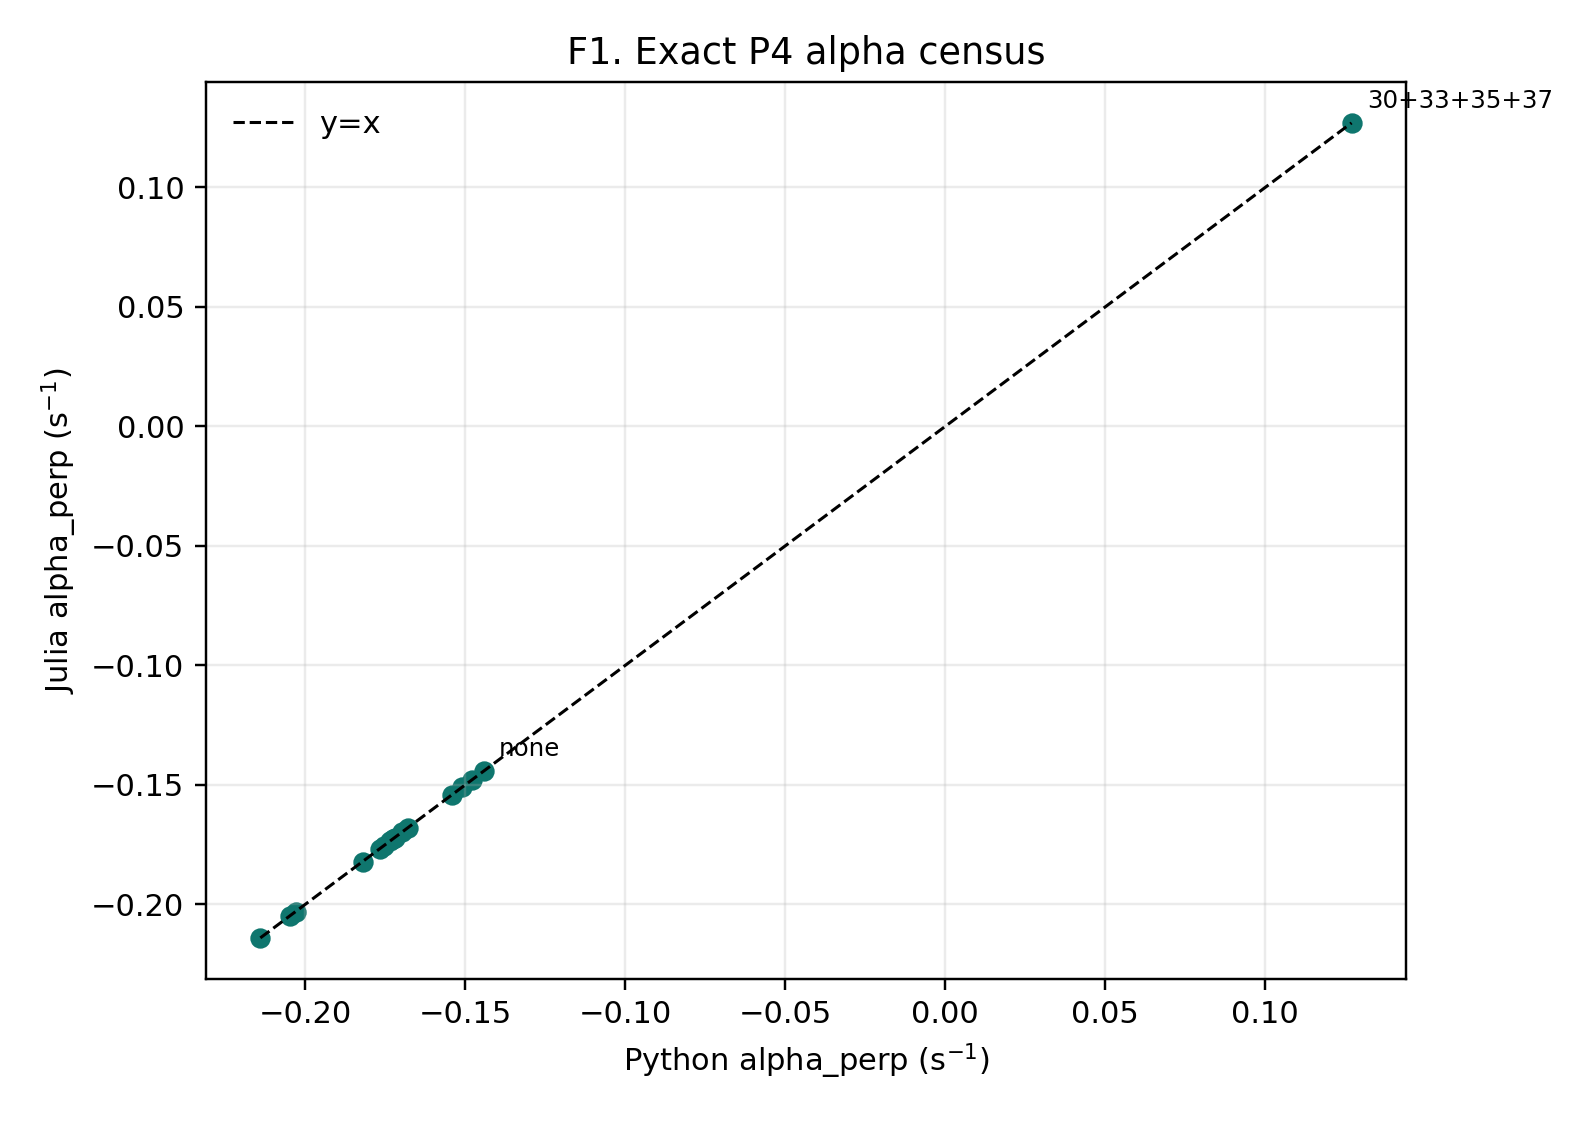
\includegraphics[width=0.82\linewidth]{../figures/TX4_F1_ALPHA_CROSSCODE.png}
\caption{All 16 alpha values: Python versus Julia.}
\end{figure}

\begin{figure}[ht]
\centering
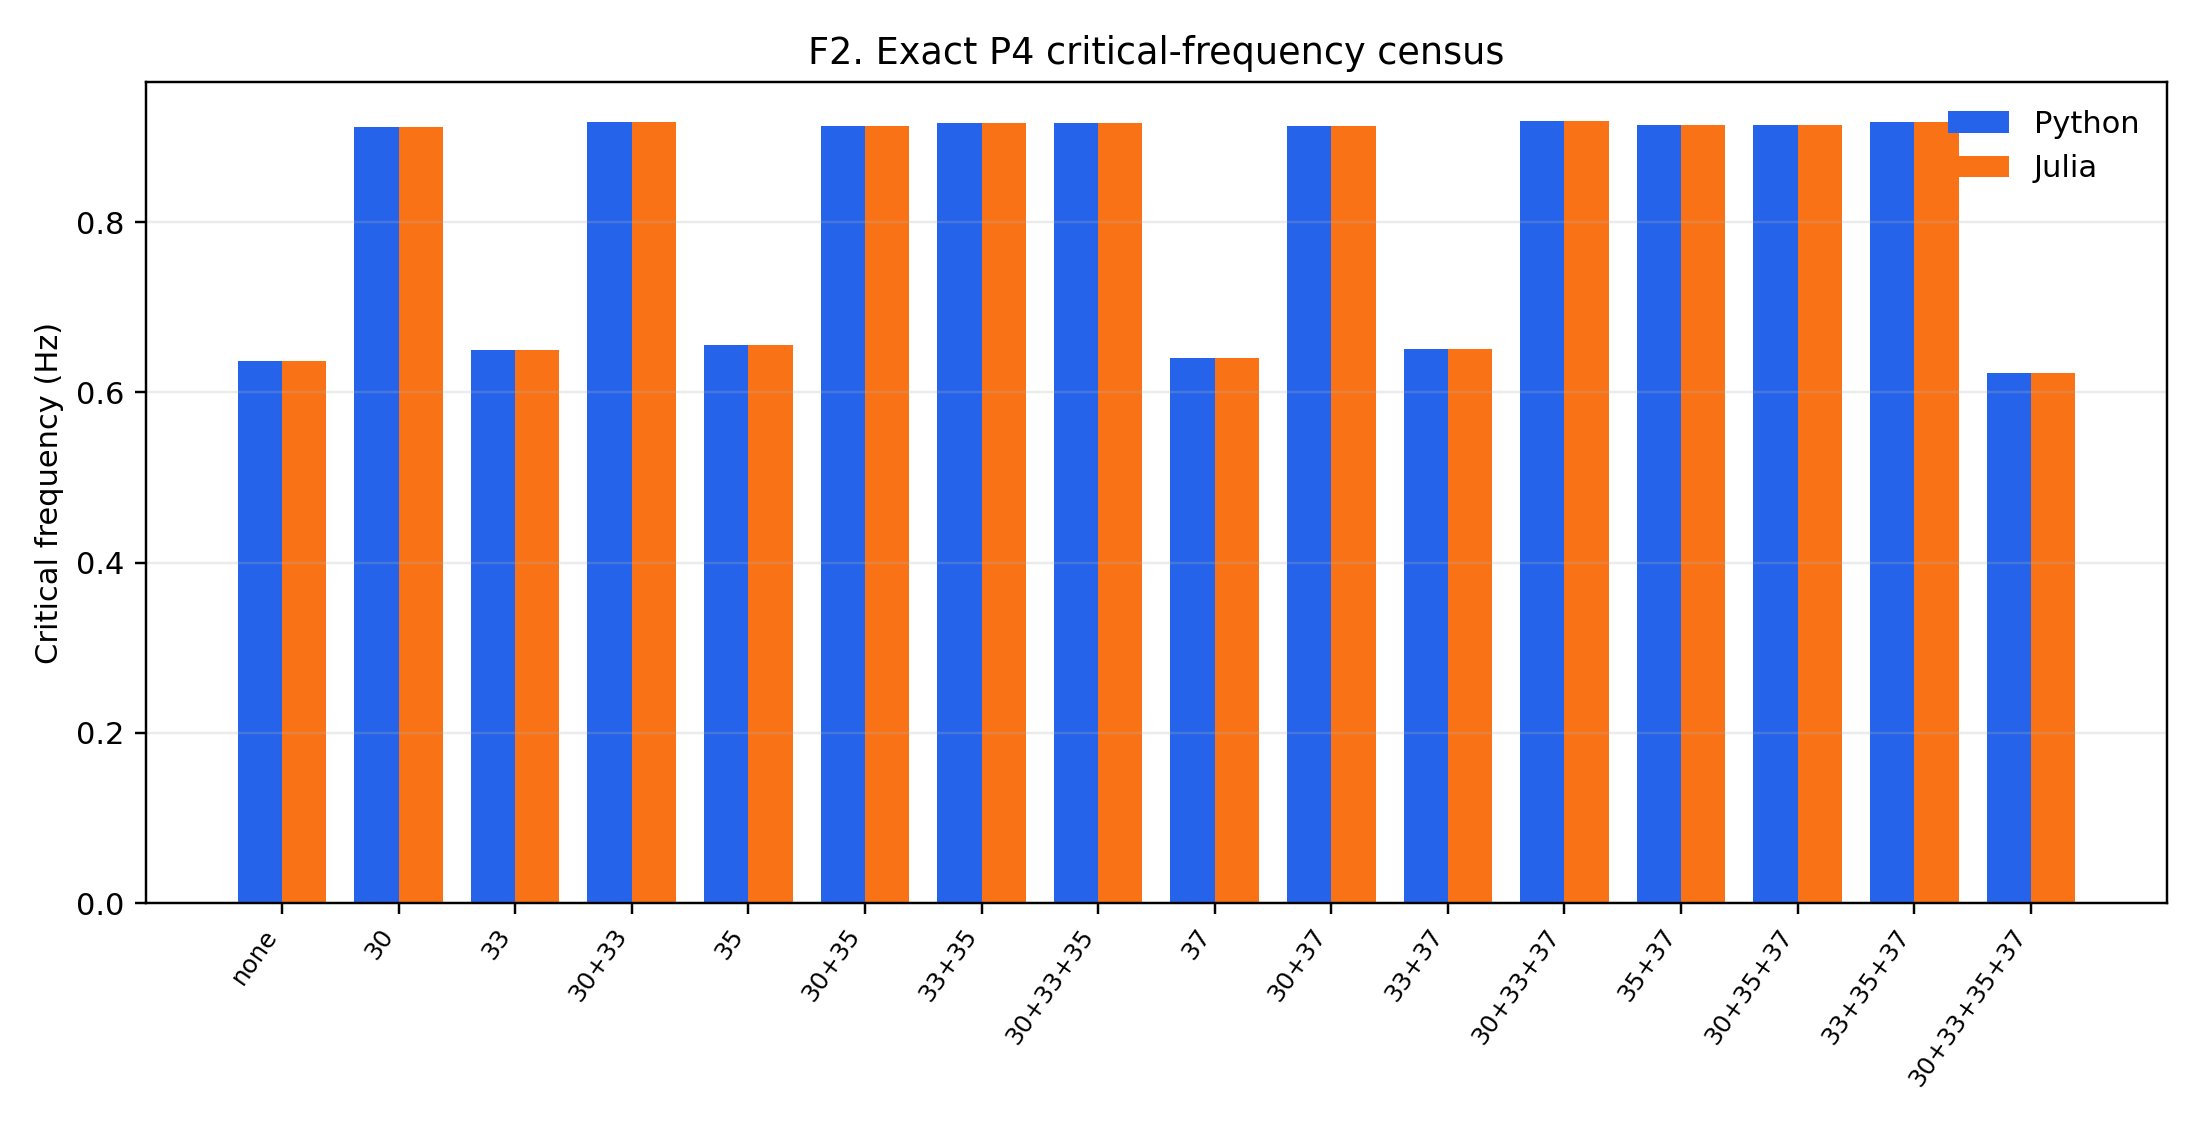
\includegraphics[width=0.98\linewidth]{../figures/TX4_F2_FREQUENCY_CROSSCODE.png}
\caption{All 16 critical frequencies.}
\end{figure}

\begin{figure}[ht]
\centering
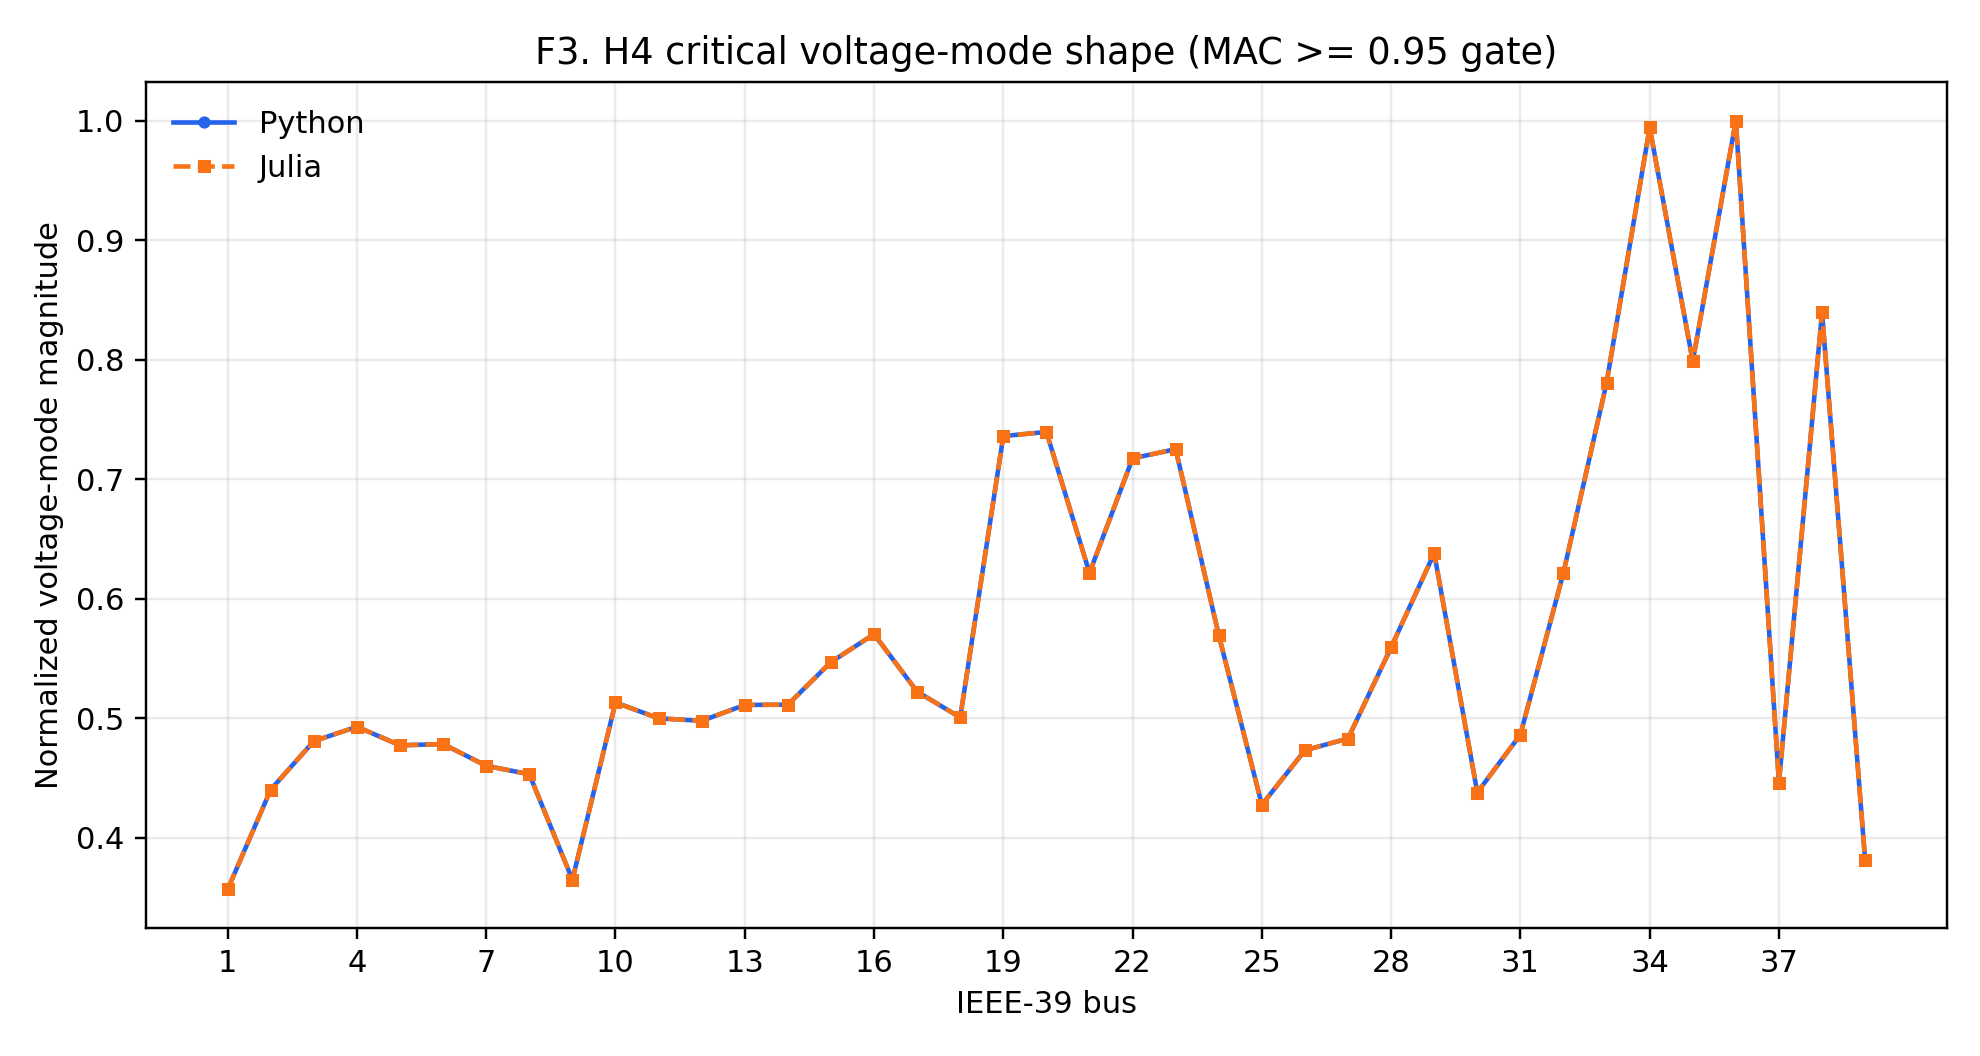
\includegraphics[width=0.98\linewidth]{../figures/TX4_F3_H4_VOLTAGE_MODE.png}
\caption{H4 critical voltage-mode magnitude by IEEE-39 bus.}
\end{figure}

\begin{figure}[ht]
\centering
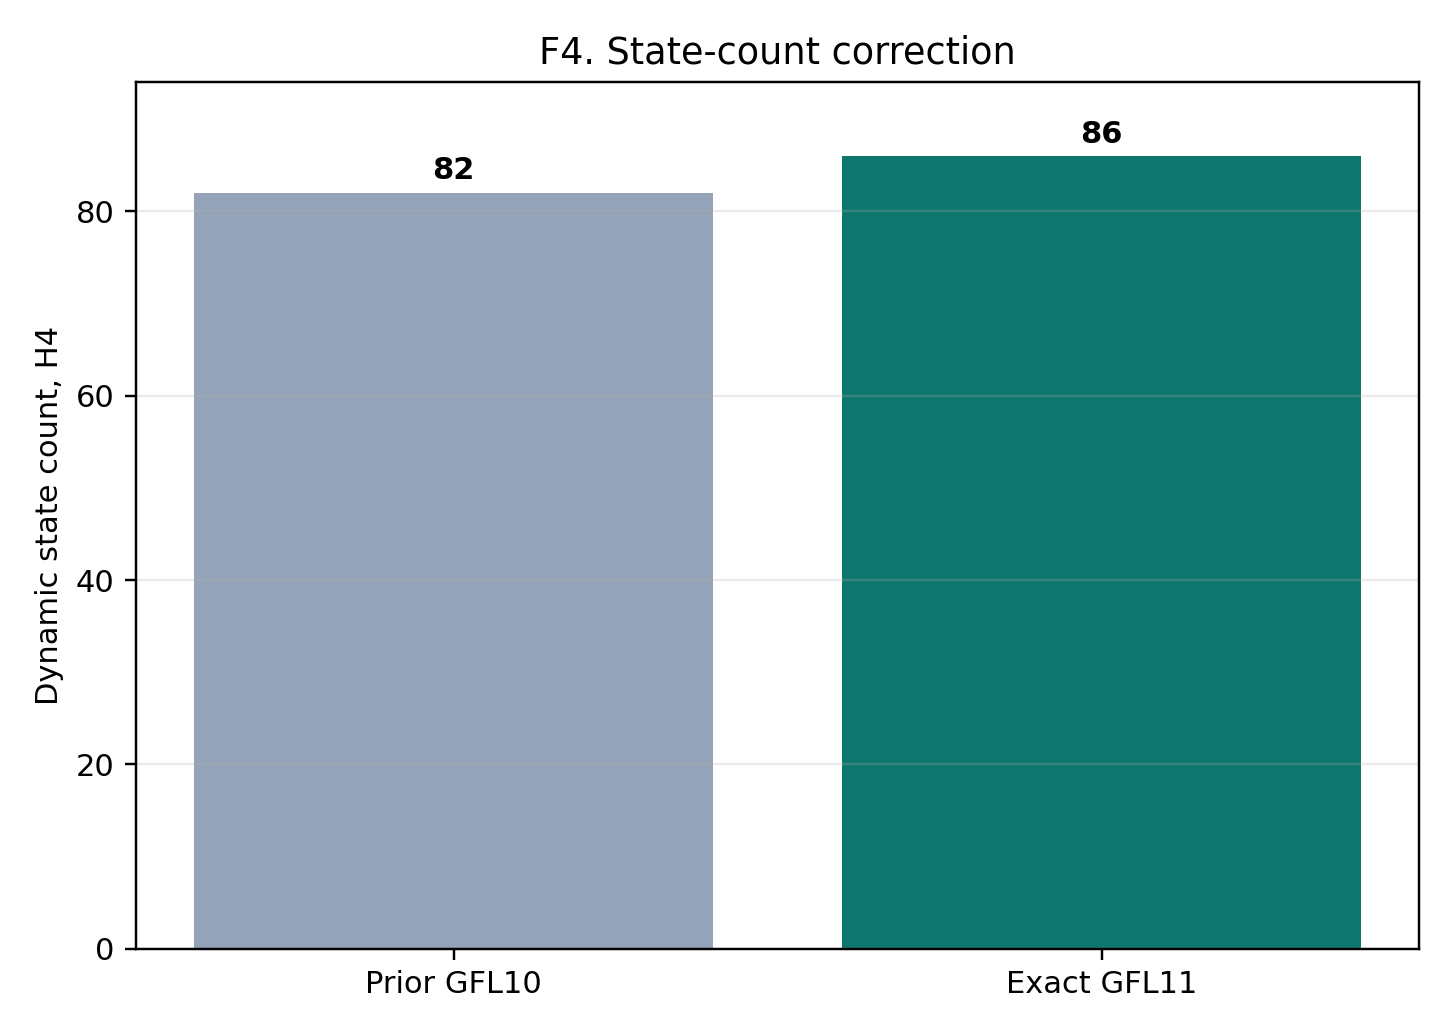
\includegraphics[width=0.72\linewidth]{../figures/TX4_F4_STATE_COUNTS.png}
\caption{Correction from prior GFL10 to exact GFL11 state count.}
\end{figure}

\section*{Evidence and limitations}

The complete numerical evidence is in the cross-code census, all-SG parity, device parity, mode-match, and state-count CSV files. The exact equations and policy are audited in the two accompanying Markdown documents.

The allowed claim is limited to cross-language reproduction of the frozen P4/GFL11 same-model spectral result for the declared reduced custom IEEE-39 DAE. It does not validate EMT behavior, a second independent dynamic model, controller saturation, protection, faults, or TPWRS submission readiness.

\section*{Reproducibility}

Branch: \texttt{research/tx4-exact-p4-julia-reproduction}. Parent: \texttt{069fa21204aa7c6f45fb44eb17e304ab99685a2b}. No push was performed.

\end{document}
